\subsubsection{「アーキテクチャ」という語の意味}
ソフトウェア工学では、「アーキテクチャ」という語が少なくとも三つの意味で使われる。

第一に、アーキテクチャは\keyterm{分野}を指す。これは、ソフトウェア集約システムを構成するための考え方、原則、過程、方法を扱う知識領域である。建築における建築学が、建物をどう構成するかを扱うのと同じように、ソフトウェアアーキテクチャは、ソフトウェア集約システムをどう構成するかを扱う。

第二に、アーキテクチャは\keyterm{活動}を指す。アーキテクチャを作る活動は、しばしば「アーキテクチャ設計」または「アーキテクティング」と呼ばれる。ソフトウェア設計は、一般にアーキテクチャ設計、高水準設計、詳細設計に分けられる。この章は、その中でも根本的な構造や重要な意思決定に関わる部分を扱う。

第三に、アーキテクチャは\keyterm{成果}を指す。つまり、あるシステムについて、主要な構成要素、関係、原則、設計判断がどのようになっているかという結果である。この成果は、アーキテクチャ記述として表される。

かつての定義では、アーキテクチャは「システムまたは構成要素の組織構造」と理解されることが多かった。しかし、現代の考え方では、単なる構造だけでは足りない。ソフトウェアには、コード構造だけでなく、実行時構造、配置構造、情報構造、開発組織との対応、運用構造など、複数の構造がある。また、アーキテクチャは環境の中のシステムとして考える必要がある。

\begin{definitionbox}
ソフトウェアアーキテクチャとは、システムの環境における根本的な概念または性質であり、構成要素、構成要素間の関係、設計と進化の原則として表れるものである。
\end{definitionbox}

この定義の要点は二つである。第一に、アーキテクチャはすべての詳細を含むものではなく、根本的なものを扱う。第二に、アーキテクチャはシステムの外側も見る。利用者、組織、外部システム、ハードウェア、法律、規制、運用環境などとの関係が重要である。

\begin{figure}[htbp]
\centering
\IfFileExists{assets/generated_figures/ch02/fig-ch02-02.png}{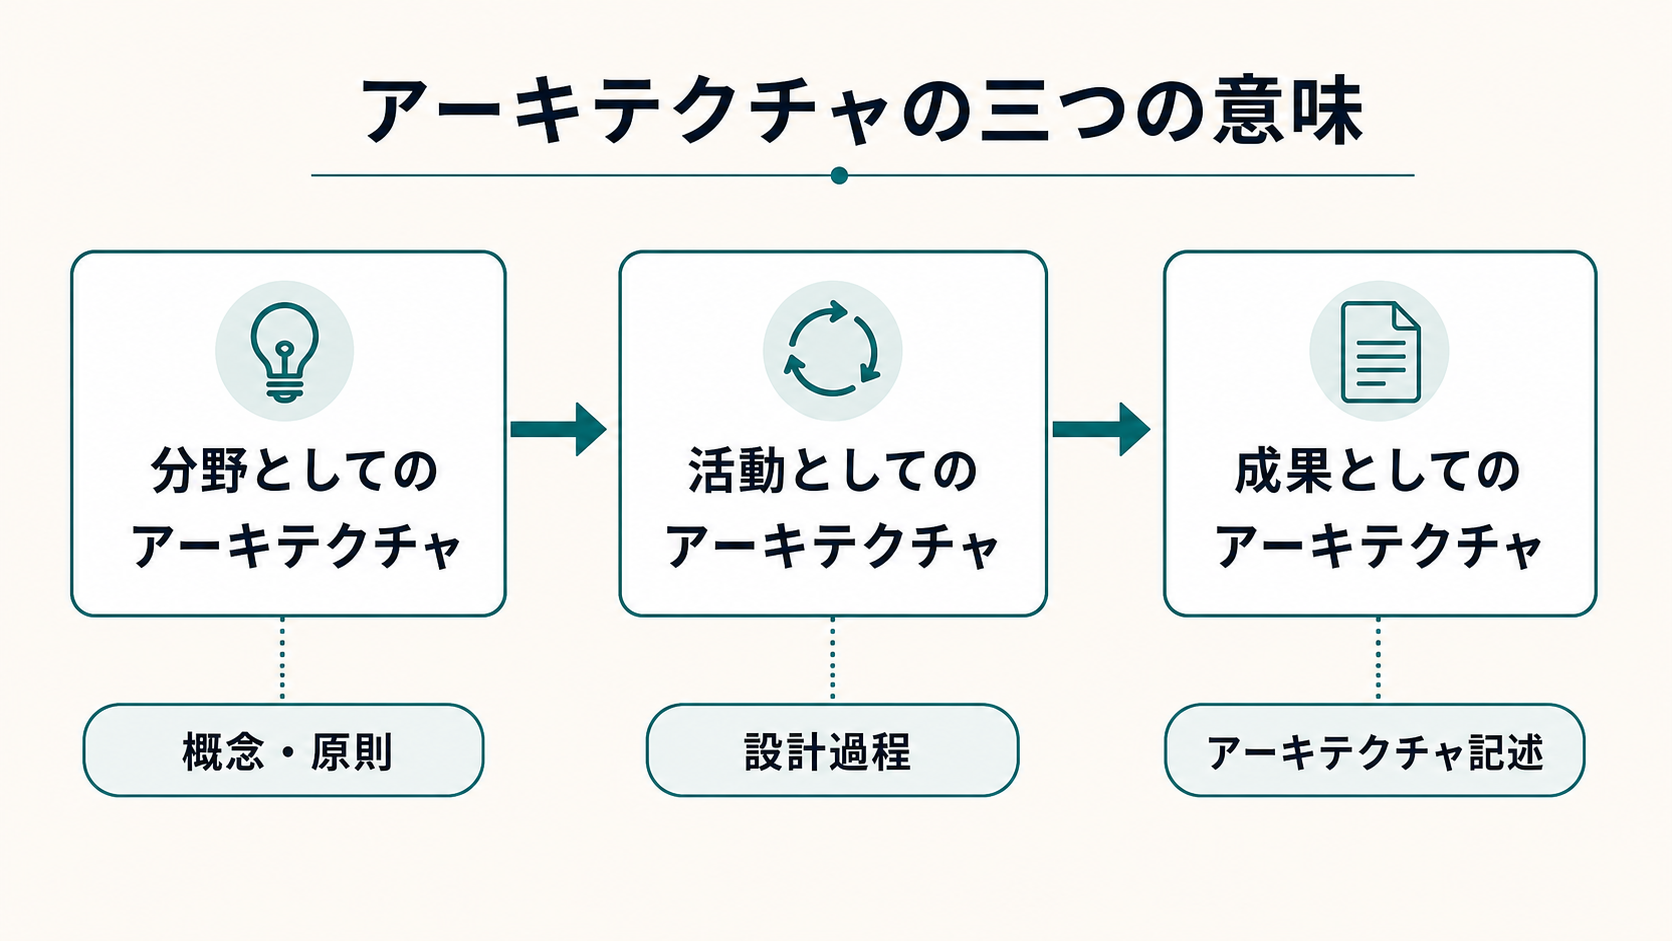
\includegraphics[width=0.96\linewidth]{assets/generated_figures/ch02/fig-ch02-02.png}}{\fbox{\parbox[c][48mm][c]{0.9\linewidth}{\centering 画像生成待ち\\アーキテクチャの三つの意味}}}
\caption{アーキテクチャの三つの意味}
\label{fig:ch02-02}
\end{figure}
